% !TeX TS-program = xelatex

\documentclass{resume}
\ResumeName{\songti  刘华强}
% 如果想插入照片，请使用以下两个库。
\usepackage{graphicx}
\usepackage{tikz}
\usepackage{enumitem}
\usepackage{xcolor}
\definecolor{myblue}{RGB}{0,48,96}
\definecolor{deepred}{RGB}{120,20,20}
% \definecolor{myblue}{RGB}{0,0,0}
% \definecolor{deepred}{RGB}{0,0,0}

\begin{document}

\begin{tikzpicture}[remember picture, overlay]
  \node[anchor=north east] at ([xshift=-0.6cm,yshift=-1.15cm]current page.north east) {
    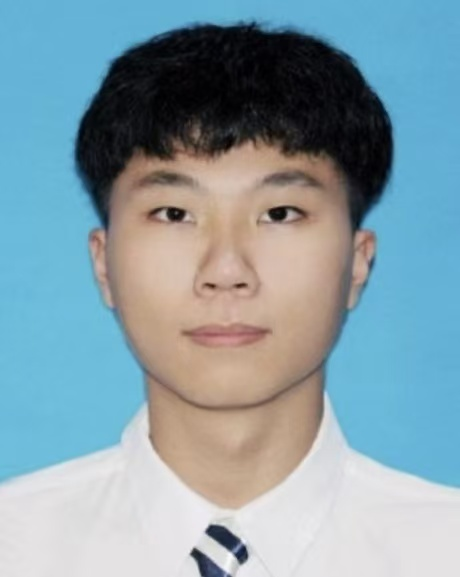
\includegraphics[width=2.4cm,height=3.2cm]{photo}
  };
\end{tikzpicture}
\small
\begin{flushleft}


\ResumeContacts{\zihao{5}
  2004/03,%
  15045468496,%
  liuhq317@163.com
}

\ResumeTitle

\vspace{0.8em}

\ResumeItem
[哈尔滨工业大学|本科生]
{\textcolor{myblue}{哈尔滨工业大学}}
[\textnormal{自动化 | 大四 | 2022.08—2026.06 }]


\textbf{学分绩：92.268}，\textbf{综合排名：9/108}，\textbf{CET-4} 480 ，\textbf{CET-6} 439 \\
\textbf{求职信息：}机器人控制算法工程师 / 具身智能相关算法岗位，随时到岗，可连续实习3个月以上，校内事务协调便利，\\可稳定投入实习工作。

\end{flushleft}

\section{\textcolor{myblue}{技术能力}}
\begin{itemize}
  \item \textbf{编程与开发}: 熟悉 \textbf{C/C++}、\textbf{Python}，具备面向真实机器人系统的代码开发、调试与工程化实现经验。
  \item \textbf{机器人平台与系统集成}: 熟悉 \textbf{Ubuntu} 开发环境，具备 \textbf{Franka} 机械臂、无人机等硬件的集成、调试与系统联调经验。
  \item \textbf{机器人开发框架}: 熟悉 \textbf{ROS2}、\textbf{MoveIt2}，能够完成机械臂运动规划、位姿控制、抓取流程集成与多模块协同开发。
  \item \textbf{机械臂相关技术}: 熟悉\textbf{机械臂运动学}与坐标变换，掌握手眼标定、逆运动学求解、轨迹规划、抓取执行流程设计。
  \item \textbf{控制与感知}: 具备\textbf{阻抗控制}、\textbf{PID控制}调试经验；熟悉视觉感知、目标分割、抓取位姿生成与筛选。
  \item \textbf{嵌入式}: 具备 \textbf{MCU (STM32)} 嵌入式开发、\textbf{FreeRTOS} 多任务系统经验，能够完成机器人相关软硬件系统的调试、优化与落地。
\end{itemize}

\section{\textcolor{myblue}{项目经历}}

\ResumeItem{\textbf{基于视觉-语言大模型的机械臂智能抓取研究}}
[\textcolor{deepred}{\ 本科毕业设计}]
[2025.06—2026.04]

\begin{itemize}
  \item 设计并实现基于 \textbf{Qwen3-VL、SAM、GraspNet、ROS2、MoveIt2} 的自然语言驱动机械臂智能抓取系统，完成从\textbf{自然语言指令理解、目标物体识别与定位、目标分割、抓取位姿生成到机械臂执行控制}的完整闭环。
  \item 搭建 \textbf{Ubuntu22.04 + ROS2} 开发环境，完成 \textbf{Franka Panda 七自由度机械臂} 控制系统设计与抓取流程集成，实现基于 \textbf{MoveIt2} 的运动规划，并设计与使用\textbf{关节空间和笛卡尔空间阻抗控制}。
  \item \textbf{\textcolor{deepred}{技术点：}}\textbf{Franka机械臂}、\textbf{视觉语言大模型}、\textbf{深度学习图像分割}、\textbf{深度学习抓取位姿生成}、\textbf{ROS2 /\ MoveIt2}、\textbf{阻抗控制}\\
\end{itemize}

\ResumeItem{\textbf{RoboMaster 全国大学生机器人大赛}}
[\textcolor{deepred}{\ 全国一等奖｜空中机器人组负责人}]
[2023.08—2025.08]

\begin{itemize}
  \item 作为\textbf{小组负责人}，负责整个赛季无人机系统研发与制作，统筹推进机械、电控与视觉三大模块协同开发，提升团队整体研发效率与项目完成质量，推动队伍成绩由\textbf{全国三等奖提升至全国一等奖}。
  \item 完成\textbf{无人机平台}设计与实现，设计 \textbf{1.6m 轴距无人机飞控系统}，基于 \textbf{DJI A3 飞控 + Onboard SDK} 实现任务规划与状态管理。
  \item 使用 \textbf{ROS2 与 C++}，结合 \textbf{FAST-LIO} 与 \textbf{激光雷达+IMU} 实现实时定位与建图，静态误差控制在 \textbf{10cm} 以内；
  \item 完成\textbf{三轴云台系统}设计与实现，熟悉\textbf{PID}及其衍生的各种控制策略，并结合视觉伺服，实现对高速移动目标的稳定跟踪和打击。
  \item \textbf{\textcolor{deepred}{技术点：}}\textbf{机器人系统设计}、\textbf{嵌入式实时控制}、\textbf{FreeRTOS}、\textbf{激光雷达与惯导融合定位}、\textbf{PID 控制}\\
\end{itemize}

\ResumeItem{\textbf{中国大学生工程实践与创新能力大赛}}
[\textcolor{deepred}{\ 全国一等奖｜电控组组长}]
[2025.01—2025.08]

\begin{itemize}
  \item 设计并实现基于\textbf{SCARA 机械臂与四麦轮底盘小车}的自动化集成系统，完成操作机构与移动平台协同工作。
  \item 独自编写覆盖 \textbf{20+ 项任务、100+ 状态} 的完整状态机控制逻辑，实现自动化任务流程控制与多阶段动作调度。
  \item 完成基于视觉系统的物料识别、定位与抓取，完成智能搬运任务，积累机械臂控制、电控开发与视觉系统联调经验。
  \item \textbf{\textcolor{deepred}{技术点：}}\textbf{机械臂与移动底盘协同控制}、\textbf{状态机设计}、\textbf{自动任务编排}、\textbf{机器人系统集成与联调}。\\
\end{itemize}

\ResumeItem{\textbf{全国大学生电子设计竞赛—无人机赛题}}
[\textcolor{deepred}{\ 全国二等奖｜队长、主力开发}]
[2024.05—2025.08]

\begin{itemize}
  \item 独立完成四旋翼无人机的\textbf{方案设计、结构搭建、硬件集成、控制程序开发与整机调试}，具备从系统设计到落地的\textbf{全流程工程开发能力}。
  \item 面向比赛任务需求，集成视觉目标识别算法，实现目标搜索、识别、跟踪与路径规划等核心功能，具备复杂机器人系统中的\textbf{问题定位、方案调整与系统优化能力}。
  \item 负责飞控\textbf{多层 PID 参数整定}与任务流程设计，提升无人机飞行稳定性、任务执行精度与现场鲁棒性。
  \item \textbf{\textcolor{deepred}{技术点：}}\textbf{无人机系统全流程设计与开发}、\textbf{硬件集成与整机调试}、\textbf{复杂系统问题定位与优化}、\textbf{飞控多层 PID 参数整定}、\textbf{控制系统测试与性能优化}。
\end{itemize}


\section{\textcolor{myblue}{荣誉奖项}}

\begin{itemize}
  \item \textbf{国家奖学金}(专业排名前 3\%)、\textbf{一等安雅奖学金}、\textbf{一等人民奖学金}、\textbf{二等人民奖学金}、\textbf{校级优秀学生}、\textbf{优秀团员}等
\end{itemize}

\section{\textcolor{myblue}{个人总结}}

\begin{itemize}
  \item 具备\textbf{真实机器人平台开发经验}，能够围绕机械臂任务完成\textbf{感知、规划、控制与执行闭环系统}的设计、实现与联调。
  \item 熟悉 \textbf{Ubuntu、C++、Python、ROS2、MoveIt2、机器人学} 及相关模块开发，具备较强的\textbf{机器人系统集成与工程落地能力}。
  \item 具备较强的\textbf{复杂任务拆解与系统联调能力}，能够面向实际机器人任务完成多模块协同开发、问题定位与流程优化。
  \item 持续关注\textbf{机器人操作、具身智能与智能控制}方向，具备扎实的工程实践基础和向\textbf{学习型机器人}方向深入发展的潜力。
\end{itemize}

\end{document}